%% Springer Nature sn-jnl template (sn-article-template, downloaded 2026-10-16), Math and Physical
%% Sciences numbered reference style. Skeleton only: section text is written by the authors.
%% Tables in tables/*.tex are generated by scripts/make_paper_assets.py from results/ -- do not edit by hand.
\documentclass[pdflatex,sn-mathphys-num]{sn-jnl}

\usepackage{graphicx}%
\usepackage{multirow}%
\usepackage{amsmath,amssymb,amsfonts}%
\usepackage{amsthm}%
\usepackage{mathrsfs}%
\usepackage[title]{appendix}%
\usepackage{xcolor}%
\usepackage{textcomp}%
\usepackage{manyfoot}%
\usepackage{booktabs}%
\usepackage{algorithm}%
\usepackage{algorithmicx}%
\usepackage{algpseudocode}%
\usepackage{listings}%

\graphicspath{{../figures/}}
\raggedbottom

\begin{document}

\title[Serverless vs Provisioned Databases Under Bursts]{A Simulation-Based Comparative Analysis of Serverless and Provisioned Cloud Relational Databases Under Burst Analytics Workloads}

%% Authors, order, emails and affiliations: pending owner decision (DECISIONS.md A2--A4).
\author*[1]{\fnm{Author} \sur{TBD}}\email{tbd@example.org}

\affil*[1]{\orgdiv{Department of Information Technology}, \orgname{TBD (pending owner confirmation)}, \orgaddress{\city{TBD}, \country{TBD}}}

\abstract{}

\keywords{serverless databases, provisioned databases, burst workloads, discrete-event simulation, cost model, PostgreSQL}

\maketitle

\section{Introduction}\label{sec:intro}

\section{Related Work}\label{sec:related}

\section{System and Workload}\label{sec:system}

\section{Simulator and Calibration}\label{sec:sim}

\begin{table}[htbp]
\centering
\footnotesize
\caption{Docker PostgreSQL calibration (seconds): warm median, warm p95 and cold first-query median per query at 1/2/4 vCPU (s1/s2/s4). Source: \texttt{results/calib\_docker.json}.}
\label{tab:calib}
\setlength{\tabcolsep}{3pt}
\begin{tabular}{lrrrrrrrrr}
\toprule
\textbf{query} & \textbf{s1 warm} & \textbf{s1 p95} & \textbf{s1 cold} & \textbf{s2 warm} & \textbf{s2 p95} & \textbf{s2 cold} & \textbf{s4 warm} & \textbf{s4 p95} & \textbf{s4 cold} \\
\midrule
Q01 & 0.3735 & 0.3838 & 0.4526 & 0.185 & 0.1864 & 0.2219 & 0.0996 & 0.1171 & 0.1222 \\
Q03 & 0.038 & 0.0392 & 0.1893 & 0.025 & 0.0266 & 0.09 & 0.0261 & 0.0264 & 0.0942 \\
Q04 & 0.0959 & 0.0976 & 0.1665 & 0.0619 & 0.0623 & 0.1156 & 0.0637 & 0.07 & 0.1158 \\
Q05 & 0.0277 & 0.0321 & 0.7059 & 0.02 & 0.0317 & 0.1359 & 0.0185 & 0.025 & 0.1099 \\
Q06 & 0.0507 & 0.0512 & 0.1146 & 0.0302 & 0.0323 & 0.0663 & 0.0199 & 0.0221 & 0.049 \\
Q10 & 0.0764 & 0.0767 & 0.152 & 0.0552 & 0.0567 & 0.1066 & 0.0347 & 0.035 & 0.0844 \\
Q12 & 0.0933 & 0.1083 & 0.164 & 0.0476 & 0.0494 & 0.0914 & 0.0275 & 0.0279 & 0.0643 \\
Q14 & 0.049 & 0.0504 & 0.1421 & 0.0323 & 0.0324 & 0.0745 & 0.0219 & 0.0231 & 0.0747 \\
\botrule
\end{tabular}
\end{table}

\begin{table}[htbp]
\centering
\footnotesize
\caption{Concurrency calibration (closed loop, 120 s per level) and fit latency $= b_q \max(1, a n / c)$: $a=2.584$, $R^2=0.956$, CPU per base second 2.147. Source: \texttt{results/calib\_contention.json}.}
\label{tab:contention}
\setlength{\tabcolsep}{3pt}
\begin{tabular}{lrrrrrrr}
\toprule
\textbf{size} & \textbf{n} & \textbf{completed} & \textbf{errors} & \textbf{CPU-s} & \textbf{ratio} & \textbf{pred} & \textbf{resid} \\
\midrule
s2 & 1 & 2158 & 0 & 229.72 & 1.0 & 1.292 & -0.292 \\
s2 & 2 & 2277 & 0 & 240.282 & 1.91 & 2.584 & -0.674 \\
s2 & 4 & 2001 & 3 & 240.542 & 4.398 & 5.168 & -0.77 \\
s2 & 8 & 1511 & 22 & 241.01 & 10.927 & 10.336 & 0.591 \\
\botrule
\end{tabular}
\end{table}


\begin{figure}[htbp]
\centering
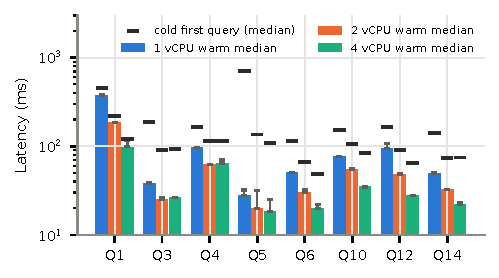
\includegraphics[width=\linewidth]{calibration_docker.pdf}
\caption{Placeholder caption. Source: \texttt{results/calib\_docker.json}.}
\label{fig:calibration}
\end{figure}

\begin{figure}[htbp]
\centering
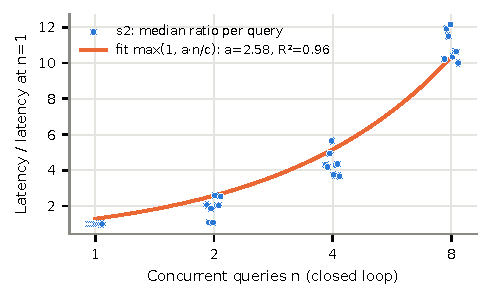
\includegraphics[width=\linewidth]{contention_fit.pdf}
\caption{Placeholder caption. Source: \texttt{results/calib\_contention.json}.}
\label{fig:contention}
\end{figure}

\section{Policies and Cost Model}\label{sec:policies}

\section{Validation}\label{sec:validation}

\begin{table}[htbp]
\centering
\footnotesize
\caption{Validation v1: sim v1 vs a real 10-min Docker s2 replay (trace seed 4242); frozen bands 25\% (p95) and 20\% (CPU-s). Source: \texttt{results/validation.json}.}
\label{tab:valv1}
\setlength{\tabcolsep}{3pt}
\begin{tabular}{lrrll}
\toprule
\textbf{metric} & \textbf{real} & \textbf{sim v1} & \textbf{error} & \textbf{pass} \\
\midrule
p95 latency (s) & 2.3358 & 0.1859 & -92.0\% & no \\
CPU-seconds & 654.7649 & 296.2695 & -54.8\% & no \\
\botrule
\end{tabular}
\end{table}

\begin{table}[htbp]
\centering
\footnotesize
\caption{Validation v2 on a new trace (seed 9191); 61 real queries failed (DiskFull). Source: \texttt{results/validation\_v2.json}.}
\label{tab:valv2}
\setlength{\tabcolsep}{3pt}
\begin{tabular}{lrrlrrll}
\toprule
\textbf{sim} & \textbf{p95 real} & \textbf{p95 sim} & \textbf{p95 err} & \textbf{CPU-s real} & \textbf{CPU-s sim} & \textbf{CPU-s err} & \textbf{pass} \\
\midrule
v1 & 1.6225 & 0.1864 & -88.5\% & 634.5695 & 291.48 & -54.1\% & no \\
v2 & 1.6225 & 2.1838 & +34.6\% & 634.5695 & 625.8179 & -1.4\% & no \\
\botrule
\end{tabular}
\end{table}


\begin{figure}[htbp]
\centering
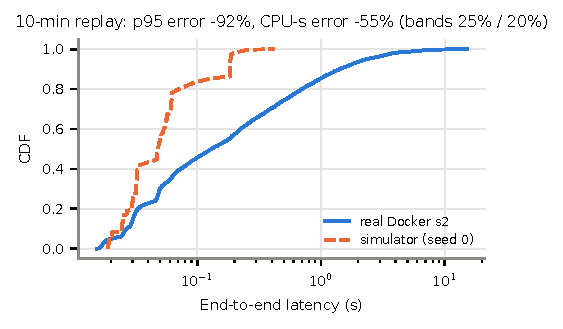
\includegraphics[width=\linewidth]{validation_sim_vs_real.pdf}
\caption{Placeholder caption. Source: \texttt{results/validation.json}.}
\label{fig:validationv1}
\end{figure}

\begin{figure}[htbp]
\centering
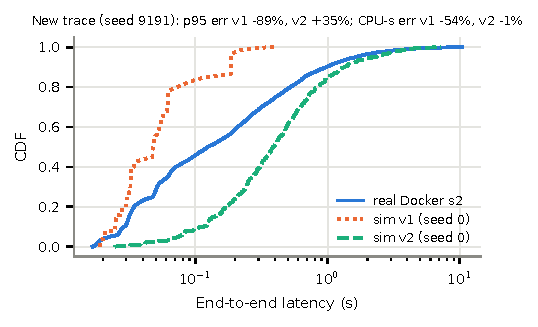
\includegraphics[width=\linewidth]{validation_v2_sim_vs_real.pdf}
\caption{Placeholder caption. Source: \texttt{results/validation\_v2.json}.}
\label{fig:validationv2}
\end{figure}

\section{Results}\label{sec:results}

\begin{table}[htbp]
\centering
\tiny\renewcommand{\arraystretch}{0.85}
\caption{Synthetic burst sweep, sim v1 (means over 10 seeds; latency not validated). p95 target 0.5 s. Source: \texttt{results/sweep.parquet}, \texttt{results/sweep.json}.}
\label{tab:sweepv1}
\setlength{\tabcolsep}{3pt}
\begin{tabular}{lllrrrrrr}
\toprule
\textbf{intensity} & \textbf{gap} & \textbf{policy} & \textbf{p95} & \textbf{p99} & \textbf{cost1k} & \textbf{vcpu\_s} & \textbf{cold} & \textbf{meets\_p95} \\
\midrule
high & long & P-peak & 0.1027 & 0.1199 & 0.0358 & 4.32e+04 & 0.0 & 1.0 \\
high & long & P-mean & 61.8166 & 69.2862 & 0.009 & 1.08e+04 & 0.0 & 0.0 \\
high & long & P-sched & 0.1027 & 0.1199 & 0.0148 & 1.782e+04 & 0.0 & 1.0 \\
high & long & S-default & 9.792 & 17.457 & 0.0208 & 8760.2327 & 7.0 & 0.0 \\
high & long & S-tuned & 0.176 & 1.8969 & 0.025 & 1.056e+04 & 0.0 & 1.0 \\
high & long & S-floor & 0.176 & 1.8969 & 0.025 & 1.056e+04 & 0.0 & 1.0 \\
high & long & S-prewarm & 0.1856 & 4.495 & 0.0213 & 8985.8638 & 1.0 & 1.0 \\
high & short & P-peak & 0.1027 & 0.1199 & 0.0124 & 4.32e+04 & 0.0 & 1.0 \\
high & short & P-mean & 0.1853 & 0.2187 & 0.0062 & 2.16e+04 & 0.0 & 1.0 \\
high & short & P-sched & 0.1027 & 0.1199 & 0.0089 & 3.114e+04 & 0.0 & 1.0 \\
high & short & S-default & 0.1655 & 1.4152 & 0.0214 & 2.608e+04 & 0.0 & 1.0 \\
high & short & S-tuned & 0.1655 & 1.4152 & 0.0214 & 2.608e+04 & 0.0 & 1.0 \\
high & short & S-floor & 0.1655 & 1.4152 & 0.0214 & 2.608e+04 & 0.0 & 1.0 \\
high & short & S-prewarm & 0.1655 & 1.4152 & 0.0214 & 2.608e+04 & 0.0 & 1.0 \\
low & long & P-peak & 0.1033 & 0.1199 & 0.4281 & 4.32e+04 & 0.0 & 1.0 \\
low & long & P-mean & 0.3749 & 0.4242 & 0.107 & 1.08e+04 & 0.0 & 1.0 \\
low & long & P-sched & 0.1033 & 0.1199 & 0.1766 & 1.782e+04 & 0.0 & 1.0 \\
low & long & S-default & 3.0002 & 14.3423 & 0.1163 & 4106.3317 & 7.0 & 0.0 \\
low & long & S-tuned & 0.3737 & 0.476 & 0.163 & 5757.525 & 0.0 & 1.0 \\
low & long & S-floor & 0.3737 & 0.476 & 0.163 & 5757.525 & 0.0 & 1.0 \\
low & long & S-prewarm & 0.3764 & 1.755 & 0.1198 & 4229.6753 & 1.0 & 1.0 \\
low & short & P-peak & 0.1015 & 0.1199 & 0.1487 & 4.32e+04 & 0.0 & 1.0 \\
low & short & P-mean & 0.3749 & 0.4235 & 0.0372 & 1.08e+04 & 0.0 & 1.0 \\
low & short & P-sched & 0.1015 & 0.1199 & 0.1072 & 3.114e+04 & 0.0 & 1.0 \\
low & short & S-default & 0.3736 & 0.4795 & 0.1144 & 1.164e+04 & 0.0 & 1.0 \\
low & short & S-tuned & 0.3736 & 0.4795 & 0.1144 & 1.164e+04 & 0.0 & 1.0 \\
low & short & S-floor & 0.3736 & 0.4795 & 0.1144 & 1.164e+04 & 0.0 & 1.0 \\
low & short & S-prewarm & 0.3736 & 0.4795 & 0.1144 & 1.164e+04 & 0.0 & 1.0 \\
mid & long & P-peak & 0.1027 & 0.1199 & 0.108 & 4.32e+04 & 0.0 & 1.0 \\
mid & long & P-mean & 0.5027 & 0.7767 & 0.027 & 1.08e+04 & 0.0 & 0.4 \\
mid & long & P-sched & 0.1027 & 0.1199 & 0.0445 & 1.782e+04 & 0.0 & 1.0 \\
mid & long & S-default & 5.0736 & 15.1834 & 0.0428 & 5993.8323 & 7.0 & 0.0 \\
mid & long & S-tuned & 0.1867 & 0.4437 & 0.0553 & 7746.05 & 0.0 & 1.0 \\
mid & long & S-floor & 0.1867 & 0.4437 & 0.0553 & 7746.05 & 0.0 & 1.0 \\
mid & long & S-prewarm & 0.2003 & 1.7573 & 0.0441 & 6183.5006 & 1.0 & 1.0 \\
mid & short & P-peak & 0.1033 & 0.1199 & 0.0372 & 4.32e+04 & 0.0 & 1.0 \\
mid & short & P-mean & 0.5072 & 0.7725 & 0.0093 & 1.08e+04 & 0.0 & 0.3 \\
mid & short & P-sched & 0.1033 & 0.1199 & 0.0268 & 3.114e+04 & 0.0 & 1.0 \\
mid & short & S-default & 0.1867 & 0.45 & 0.0429 & 1.744e+04 & 0.0 & 1.0 \\
mid & short & S-tuned & 0.1867 & 0.45 & 0.0429 & 1.744e+04 & 0.0 & 1.0 \\
mid & short & S-floor & 0.1867 & 0.45 & 0.0429 & 1.744e+04 & 0.0 & 1.0 \\
mid & short & S-prewarm & 0.1867 & 0.45 & 0.0429 & 1.744e+04 & 0.0 & 1.0 \\
\botrule
\end{tabular}
\end{table}

\clearpage
\begin{table}[htbp]
\centering
\tiny\renewcommand{\arraystretch}{0.85}
\caption{Cost per 1,000 queries (USD), sim v1 vs sim v2 (headline: v2), seeds 0--9; /P-peak = ratio to P-peak in the same cell; NV = not validated. Source: \texttt{results/sweep.parquet}, \texttt{results/sweep\_v2.parquet}.}
\label{tab:costv1v2}
\setlength{\tabcolsep}{3pt}
\begin{tabular}{lllrrrrr}
\toprule
\textbf{intensity} & \textbf{gap} & \textbf{policy} & \textbf{cost1k v1} & \textbf{cost1k v2} & \textbf{/P-peak v1} & \textbf{/P-peak v2} & \textbf{p95 v2 (NV)} \\
\midrule
high & long & P-peak & 0.0358 & 0.0358 & 1.0 & 1.0 & 0.1285 \\
high & long & P-mean & 0.009 & 0.009 & 0.25 & 0.25 & 597.5216 \\
high & long & P-sched & 0.0148 & 0.0148 & 0.413 & 0.413 & 0.1285 \\
high & long & S-default & 0.0208 & 0.0359 & 0.579 & 1.001 & 33.7881 \\
high & long & S-tuned & 0.025 & 0.031 & 0.699 & 0.864 & 3.73 \\
high & long & S-floor & 0.025 & 0.031 & 0.699 & 0.864 & 3.73 \\
high & long & S-prewarm & 0.0213 & 0.0289 & 0.594 & 0.806 & 8.4747 \\
high & short & P-peak & 0.0124 & 0.0124 & 1.0 & 1.0 & 0.1286 \\
high & short & P-mean & 0.0062 & 0.0062 & 0.5 & 0.5 & 2.2956 \\
high & short & P-sched & 0.0089 & 0.0089 & 0.721 & 0.721 & 0.1286 \\
high & short & S-default & 0.0214 & 0.0269 & 1.725 & 2.171 & 0.9855 \\
high & short & S-tuned & 0.0214 & 0.0269 & 1.725 & 2.171 & 0.9855 \\
high & short & S-floor & 0.0214 & 0.0269 & 1.725 & 2.171 & 0.9855 \\
high & short & S-prewarm & 0.0214 & 0.0269 & 1.725 & 2.171 & 0.9855 \\
low & long & P-peak & 0.4281 & 0.4281 & 1.0 & 1.0 & 0.1052 \\
low & long & P-mean & 0.107 & 0.107 & 0.25 & 0.25 & 0.9919 \\
low & long & P-sched & 0.1766 & 0.1766 & 0.413 & 0.413 & 0.1052 \\
low & long & S-default & 0.1163 & 0.246 & 0.272 & 0.575 & 10.9328 \\
low & long & S-tuned & 0.163 & 0.1942 & 0.381 & 0.454 & 0.5835 \\
low & long & S-floor & 0.163 & 0.1942 & 0.381 & 0.454 & 0.5835 \\
low & long & S-prewarm & 0.1198 & 0.1689 & 0.28 & 0.394 & 0.895 \\
low & short & P-peak & 0.1487 & 0.1487 & 1.0 & 1.0 & 0.1045 \\
low & short & P-mean & 0.0372 & 0.0372 & 0.25 & 0.25 & 0.9947 \\
low & short & P-sched & 0.1072 & 0.1072 & 0.721 & 0.721 & 0.1045 \\
low & short & S-default & 0.1144 & 0.1464 & 0.77 & 0.985 & 0.5491 \\
low & short & S-tuned & 0.1144 & 0.1464 & 0.77 & 0.985 & 0.5491 \\
low & short & S-floor & 0.1144 & 0.1464 & 0.77 & 0.985 & 0.5491 \\
low & short & S-prewarm & 0.1144 & 0.1464 & 0.77 & 0.985 & 0.5491 \\
mid & long & P-peak & 0.108 & 0.108 & 1.0 & 1.0 & 0.1058 \\
mid & long & P-mean & 0.027 & 0.027 & 0.25 & 0.25 & 29.1859 \\
mid & long & P-sched & 0.0445 & 0.0445 & 0.413 & 0.413 & 0.1058 \\
mid & long & S-default & 0.0428 & 0.1046 & 0.396 & 0.969 & 18.9218 \\
mid & long & S-tuned & 0.0553 & 0.0695 & 0.512 & 0.644 & 0.4569 \\
mid & long & S-floor & 0.0553 & 0.0695 & 0.512 & 0.644 & 0.4569 \\
mid & long & S-prewarm & 0.0441 & 0.0676 & 0.409 & 0.626 & 1.0634 \\
mid & short & P-peak & 0.0372 & 0.0372 & 1.0 & 1.0 & 0.1058 \\
mid & short & P-mean & 0.0093 & 0.0093 & 0.25 & 0.25 & 30.0899 \\
mid & short & P-sched & 0.0268 & 0.0268 & 0.721 & 0.721 & 0.1058 \\
mid & short & S-default & 0.0429 & 0.0572 & 1.153 & 1.539 & 0.3773 \\
mid & short & S-tuned & 0.0429 & 0.0572 & 1.153 & 1.539 & 0.3773 \\
mid & short & S-floor & 0.0429 & 0.0572 & 1.153 & 1.539 & 0.3773 \\
mid & short & S-prewarm & 0.0429 & 0.0572 & 1.153 & 1.539 & 0.3773 \\
\botrule
\end{tabular}
\end{table}

\begin{table}[htbp]
\centering
\footnotesize
\caption{S-tuned (sim v2): timeout chosen on seeds 0--9, scored on held-out seeds 10--19. Source: \texttt{results/sweep\_v2.parquet}.}
\label{tab:heldout}
\setlength{\tabcolsep}{3pt}
\begin{tabular}{lrrrrr}
\toprule
\textbf{cell} & \textbf{tau (s)} & \textbf{cost1k 0-9} & \textbf{cost1k 10-19} & \textbf{/P-peak 10-19} & \textbf{p95 10-19 (NV)} \\
\midrule
high/long & 1800 & 0.031 & 0.0307 & 0.853 & 3.6943 \\
high/short & 300 & 0.0269 & 0.0268 & 2.161 & 0.9039 \\
low/long & 1800 & 0.1942 & 0.1982 & 0.453 & 0.6066 \\
low/short & 300 & 0.1464 & 0.1474 & 0.986 & 0.5829 \\
mid/long & 1800 & 0.0695 & 0.0701 & 0.647 & 0.4352 \\
mid/short & 300 & 0.0572 & 0.0577 & 1.547 & 0.3719 \\
\botrule
\end{tabular}
\end{table}

\begin{table}[htbp]
\centering
\footnotesize
\caption{Redset replay, sim v1 (instance 1, 2024-04-10, 28615 queries; means over 10 seeds; latency not validated). Source: \texttt{results/redset\_sweep.json}, \texttt{results/redset\_trace.json}.}
\label{tab:redsetv1}
\setlength{\tabcolsep}{3pt}
\begin{tabular}{lrrrrr}
\toprule
\textbf{policy} & \textbf{p95\_s} & \textbf{p99\_s} & \textbf{compute\_vcpu\_s} & \textbf{cost\_per\_1k\_usd} & \textbf{cold\_starts} \\
\midrule
P-peak & 0.1047 & 0.1199 & 3.456e+05 & 0.2818 & 0.0 \\
P-mean & 1416.9298 & 1495.5244 & 8.64e+04 & 0.0705 & 0.0 \\
P-sched & 0.1047 & 0.1199 & 9.72e+04 & 0.0793 & 0.0 \\
S-default & 0.1152 & 0.1553 & 5393.8394 & 0.0126 & 1.0 \\
S-tuned & 0.1152 & 0.1553 & 5152.9394 & 0.012 & 1.0 \\
S-floor & 0.1116 & 0.142 & 2.651e+04 & 0.0618 & 0.0 \\
S-prewarm & 0.1152 & 0.1553 & 5393.8394 & 0.0126 & 1.0 \\
\botrule
\end{tabular}
\end{table}

\begin{table}[htbp]
\centering
\footnotesize
\caption{Redset cost per 1,000 queries, sim v1 vs sim v2; S-tuned $\tau$ (v2) = 300 s. Source: \texttt{results/redset\_sweep.json}, \texttt{results/redset\_sweep\_v2.json}.}
\label{tab:redsetcost}
\setlength{\tabcolsep}{3pt}
\begin{tabular}{lrrrrr}
\toprule
\textbf{policy} & \textbf{cost1k v1} & \textbf{cost1k v2} & \textbf{/P-peak v1} & \textbf{/P-peak v2} & \textbf{p95 v2 (NV)} \\
\midrule
P-peak & 0.2818 & 0.2818 & 1.0 & 1.0 & 0.2594 \\
P-mean & 0.0705 & 0.0705 & 0.25 & 0.25 & 5754.1977 \\
P-sched & 0.0793 & 0.0793 & 0.281 & 0.281 & 0.2594 \\
S-default & 0.0126 & 0.0139 & 0.045 & 0.049 & 10.7539 \\
S-tuned & 0.012 & 0.0139 & 0.043 & 0.049 & 10.7539 \\
S-floor & 0.0618 & 0.0628 & 0.219 & 0.223 & 0.2656 \\
S-prewarm & 0.0126 & 0.0139 & 0.045 & 0.049 & 10.7539 \\
\botrule
\end{tabular}
\end{table}

\begin{table}[htbp]
\centering
\footnotesize
\caption{Redset P-mean overload check. Source: \texttt{results/redset\_overload\_check.json}.}
\label{tab:overload}
\setlength{\tabcolsep}{3pt}
\begin{tabular}{ll}
\toprule
\textbf{quantity} & \textbf{value} \\
\midrule
P-mean size (vCPU) / servers & 1.0 / 1 \\
capacity (q/s) & 9.94 \\
rho, day mean & 0.033 \\
rho, peak hour (22) & 0.799 \\
rho, max minute & 3.04 \\
minutes with rho > 1 & 21 \\
max fluid backlog (queries) & 14344.0 \\
backlog drain (s) & 1442.3 \\
queue unbounded in overload minutes & True \\
sim v1 P-mean p95 (s) & 1416.9 \\
\botrule
\end{tabular}
\end{table}

\begin{table}[htbp]
\centering
\footnotesize
\caption{Statistics file index: mean, std, bootstrap 95\% CI and Wilcoxon signed-rank vs P-peak (paired by seed) per source, cell, policy and metric. Source: \texttt{results/stats.csv}.}
\label{tab:stats}
\setlength{\tabcolsep}{3pt}
\begin{tabular}{lrrr}
\toprule
\textbf{source} & \textbf{rows} & \textbf{policies} & \textbf{metrics} \\
\midrule
redset & 42 & 7 & 6 \\
redset\_v2 & 42 & 7 & 6 \\
redset\_v2\_heldout & 42 & 7 & 6 \\
sweep & 252 & 7 & 6 \\
sweep\_v2 & 252 & 7 & 6 \\
sweep\_v2\_heldout & 252 & 7 & 6 \\
\botrule
\end{tabular}
\end{table}


\begin{figure}[htbp]
\centering
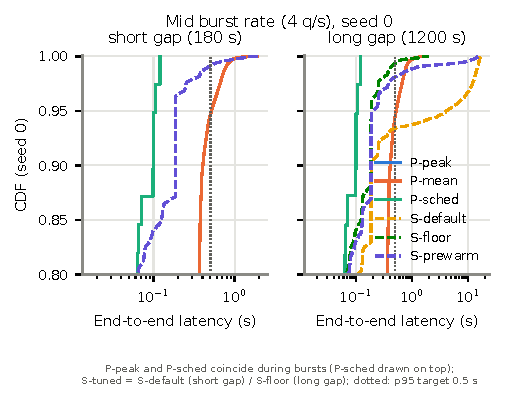
\includegraphics[width=\linewidth]{latency_cdf.pdf}
\caption{Placeholder caption. Source: \texttt{results/sweep\_latency\_seed0.parquet}.}
\label{fig:latencycdf}
\end{figure}

\begin{figure}[htbp]
\centering
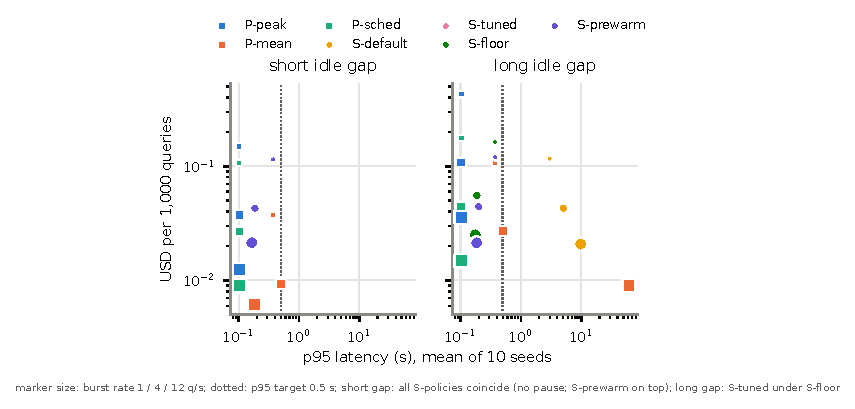
\includegraphics[width=\linewidth]{cost_vs_p95.pdf}
\caption{Placeholder caption. Source: \texttt{results/sweep.parquet}.}
\label{fig:paretov1}
\end{figure}

\begin{figure}[htbp]
\centering
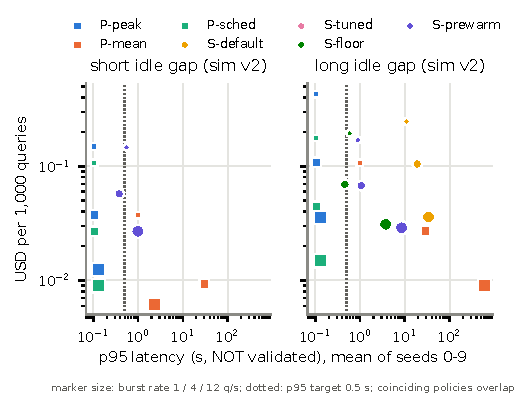
\includegraphics[width=\linewidth]{cost_vs_p95_v2.pdf}
\caption{Placeholder caption. Source: \texttt{results/sweep\_v2.parquet}.}
\label{fig:paretov2}
\end{figure}

\begin{figure}[htbp]
\centering
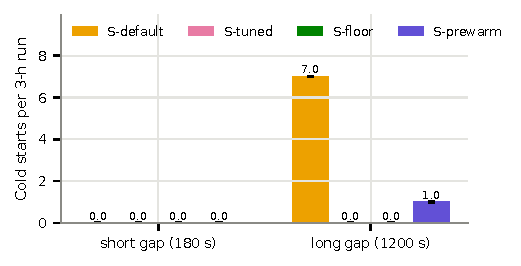
\includegraphics[width=\linewidth]{cold_starts_by_gap.pdf}
\caption{Placeholder caption. Source: \texttt{results/sweep.parquet}.}
\label{fig:coldstarts}
\end{figure}

\begin{figure}[htbp]
\centering
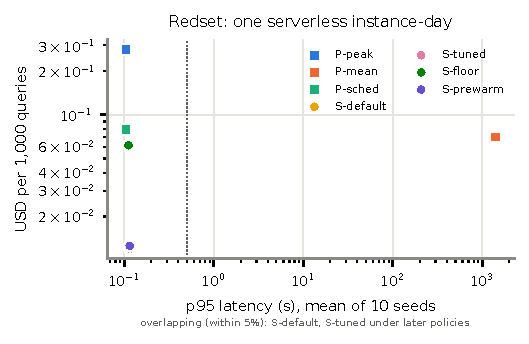
\includegraphics[width=\linewidth]{redset_cost_vs_p95.pdf}
\caption{Placeholder caption. Source: \texttt{results/redset\_sweep.parquet}.}
\label{fig:redset}
\end{figure}

\section{Threats to Validity}\label{sec:threats}

\section{Conclusion}\label{sec:conclusion}

\backmatter

\section*{Declarations}

%% All references are listed until the text cites them.
\nocite{*}
\bibliography{refs}

\end{document}
